\documentclass[10pt]{article}
\usepackage[a4paper,bindingoffset=0.2in,%
            left=0.15in,right=0.2in,top=0.3in,bottom=0.3in,%
            footskip=.25in]{geometry}

\usepackage{AFSA}

%----------------------------------------------------------------------------------------------
\title{\vspace{-2cm}\textbf{اختلاف قوت و قضایای کیسی}}
\author{ایمان قادر و مهران طلایی}
\date{\today}

%-------------------------------------------------------------------------------------------------
\pagestyle{fancy}
\fancyhf{}
\cfoot{\thepage}
%\chead{\Large \textbf{عنــــــــوان}}
\lhead{\textbf{ایمان قادر و مهران طلایی}}
\rhead{\textbf{عنوان}}


%-------------------------------Beginning------------------------------------
\begin{document}
\maketitle


\begin{abstract}
قضیه کیسی از قضایای کلاسیک و پر استفاده در هندسه است که با توجه به کمبود متریال آموزشی در حیطه این مبحث ولی کاربرد زیاد آن، به گرد آوری این مقاله روی آوردیم که شامل تعاریف و قضایای مورد نیاز و همینطوری از هر بخش مثال هایی مطرح شده اند که به یادگیری هرچه بیشتر کمک میکنند. و در انتها تمرین هایی برای دست ورزی و خودآزمایی قرار داده شده است.
\end{abstract}

ابتدا با یک تعریف شروع میکنیم:
\De{\AfterDefenition
تابع اختلاف قوت نقطه $P$ نسبت به دو دایره $\omega_1$ و $\omega_2$ را به شکل زیر تعریف میکنیم:
\[\mathbf{P}(P,\omega_1,\omega_2)=Pow_{\omega_1}^P -Pow_{\omega_2}^P\]
}





\section{صورت قضیه کیسی (اختلاف قوت)}

\Th{
\AfterTheorem
فرض کنید که دوایر $\omega_1$ و $\omega_2$ به مراکز $O_1$ و $O_2$ در صفحه هستند و خط $l$ محور اصلی این دو دایره است و نقطه $P$ نقطه ای در صفحه $\omega_1$ و $\omega_2$ است. آنوقت رابطه زیر برقرار است:
\[\mathbf{P}(P,\omega_1,\omega_2)=2dist(P,l) \overline{O_1O_2} \]
}

\Proof{
دوایر $\omega_1(O_1,r_1)$ و  $\omega_2(O_2,r_2)$ را در نظر بگیرید. و $A$ و $D$  به ترتیب پاهای عمود از $P$ بر محور اصلی و خط المرکزین این دو دایره هستند. 

\begin{figure}[!htb]
    \centering
    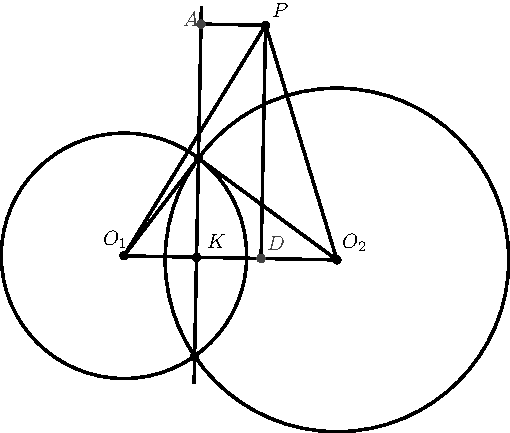
\includegraphics[width=0.5\linewidth]{Figures/caseypro.pdf}
    % \caption{Caption}
    % \label{fig:enter-label}
\end{figure}

حال داریم:
\begin{align*}
Pow_{\omega_1}^P-Pow_{\omega_2}^P &= PO_1^2-r_1^2-PO_2^2+r_2^2 \\
&= DO_1^2-DO_2^2+r_2^2-r_1^2 \\
&=(DO_1-DO_2)\overline{O_1O_2}+KO_1^2-KO_2^2\\
&=(DO_1-DO_2)\overline{O_1O_2}+(KO_1-KO_2)\overline{O_1O_2} \\
&=(DO_1-DO_2+KO_1-KO_2)\overline{O_1O_2}\\
&=2 \overline{PA} \thickspace\overline{O_1O_2} \thickspace 
\end{align*}
}


\Ex{
دایره $\omega'$ دایره ای به مرکز $O'$  به طور کامل درون دایره $\omega$ و مرکز $O$ قرار دارد. نقاط $A$ و $B$ به گونه ای بر روی دایره $\omega$ قرار دارند که  $\overline{AB}$ بر $\omega'$ مماس است. دایره $\Omega$  را دایره محیطی $\triangle{O'AB}$ در نظر بگیرید. خط $\overline{AB}$ را با حفظ جهت حرکت میدهیم مکان هندسی مرکز $\Omega$ را بیابید.
}

\Proof{

مرکز $\Omega$ را $O''$ مینامیم.

\begin{figure}[!htb]
    \centering
    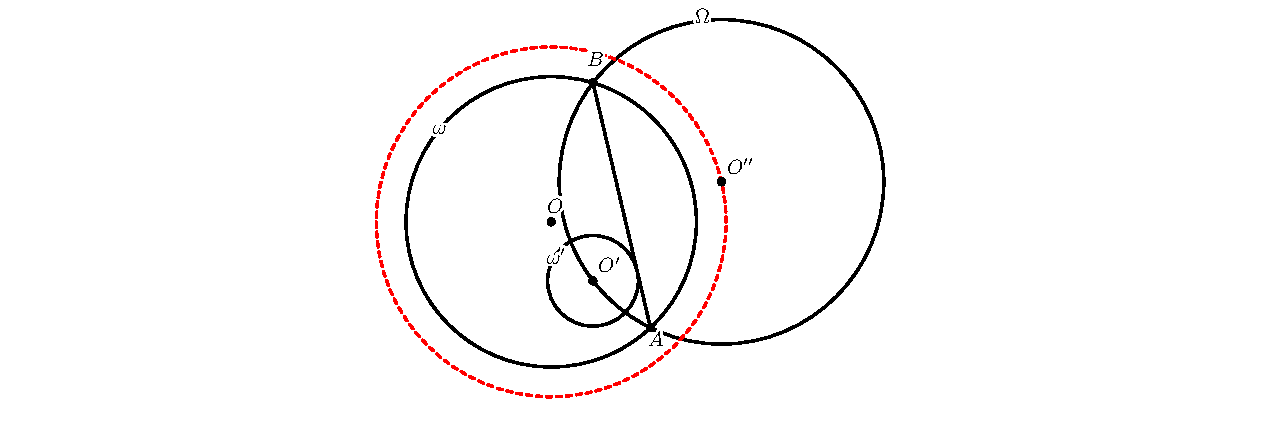
\includegraphics[width=\linewidth]{Figures/ncavenye.pdf}
    % \caption{Caption}
    % \label{fig:enter-label}
\end{figure}

حال $\mathbf{P}(O',\omega,\Omega)$ را محاسبه میکنیم:
\begin{align*}
\mathbf{P}(O',\omega,\Omega)=Pow_{\omega}^{O'}-Pow_{\Omega}^{O'}&=2 R_{\omega'} \overline{OO''}\\
\leftrightarrow \frac{Pow_{\omega}^{O'}-0}{2 R_{\omega'}}&=\overline{OO''}
\end{align*}
بنابر این طول $OO''$ ثابت است و این نتیجه میدهد که مکان هندسی $O''$ دایره ای است به مرکز $O$ و شعاع $\frac{Pow_{\omega}^{O'}}{2 R_{\omega'}}$ .

}


\newpage
\Ex{
 $\omega_B$ و $\omega_C$ دوایر محاطی خارجی مثلث $\triangle{ABC}$ هستند. دایره $\omega_B'$ با دایره $\omega_B$ نسبت به وسط $AC$ متقارن هستند و دایره $\omega_C'$ با دایره $\omega_C$ نسبت به وسط $AB$ متقارن هستند. اثبات کنید که محور اصلی  $\omega_B'$ و  $\omega_C'$ محیط مثلث را نصف میکن.  
({روسیه 2005})
}

\Proof{
 دایره محاطی مثلث را $\omega$ بنامید و محل تماس $\omega_A$ با خط $BC$ را $D$ در نظر میگیریم حال اثبات میکنیم که خط $AD$ محور اصلی دو دایره $\omega_B'$ و $\omega_C'$ است.

 \begin{figure}[!ht]
     \centering
     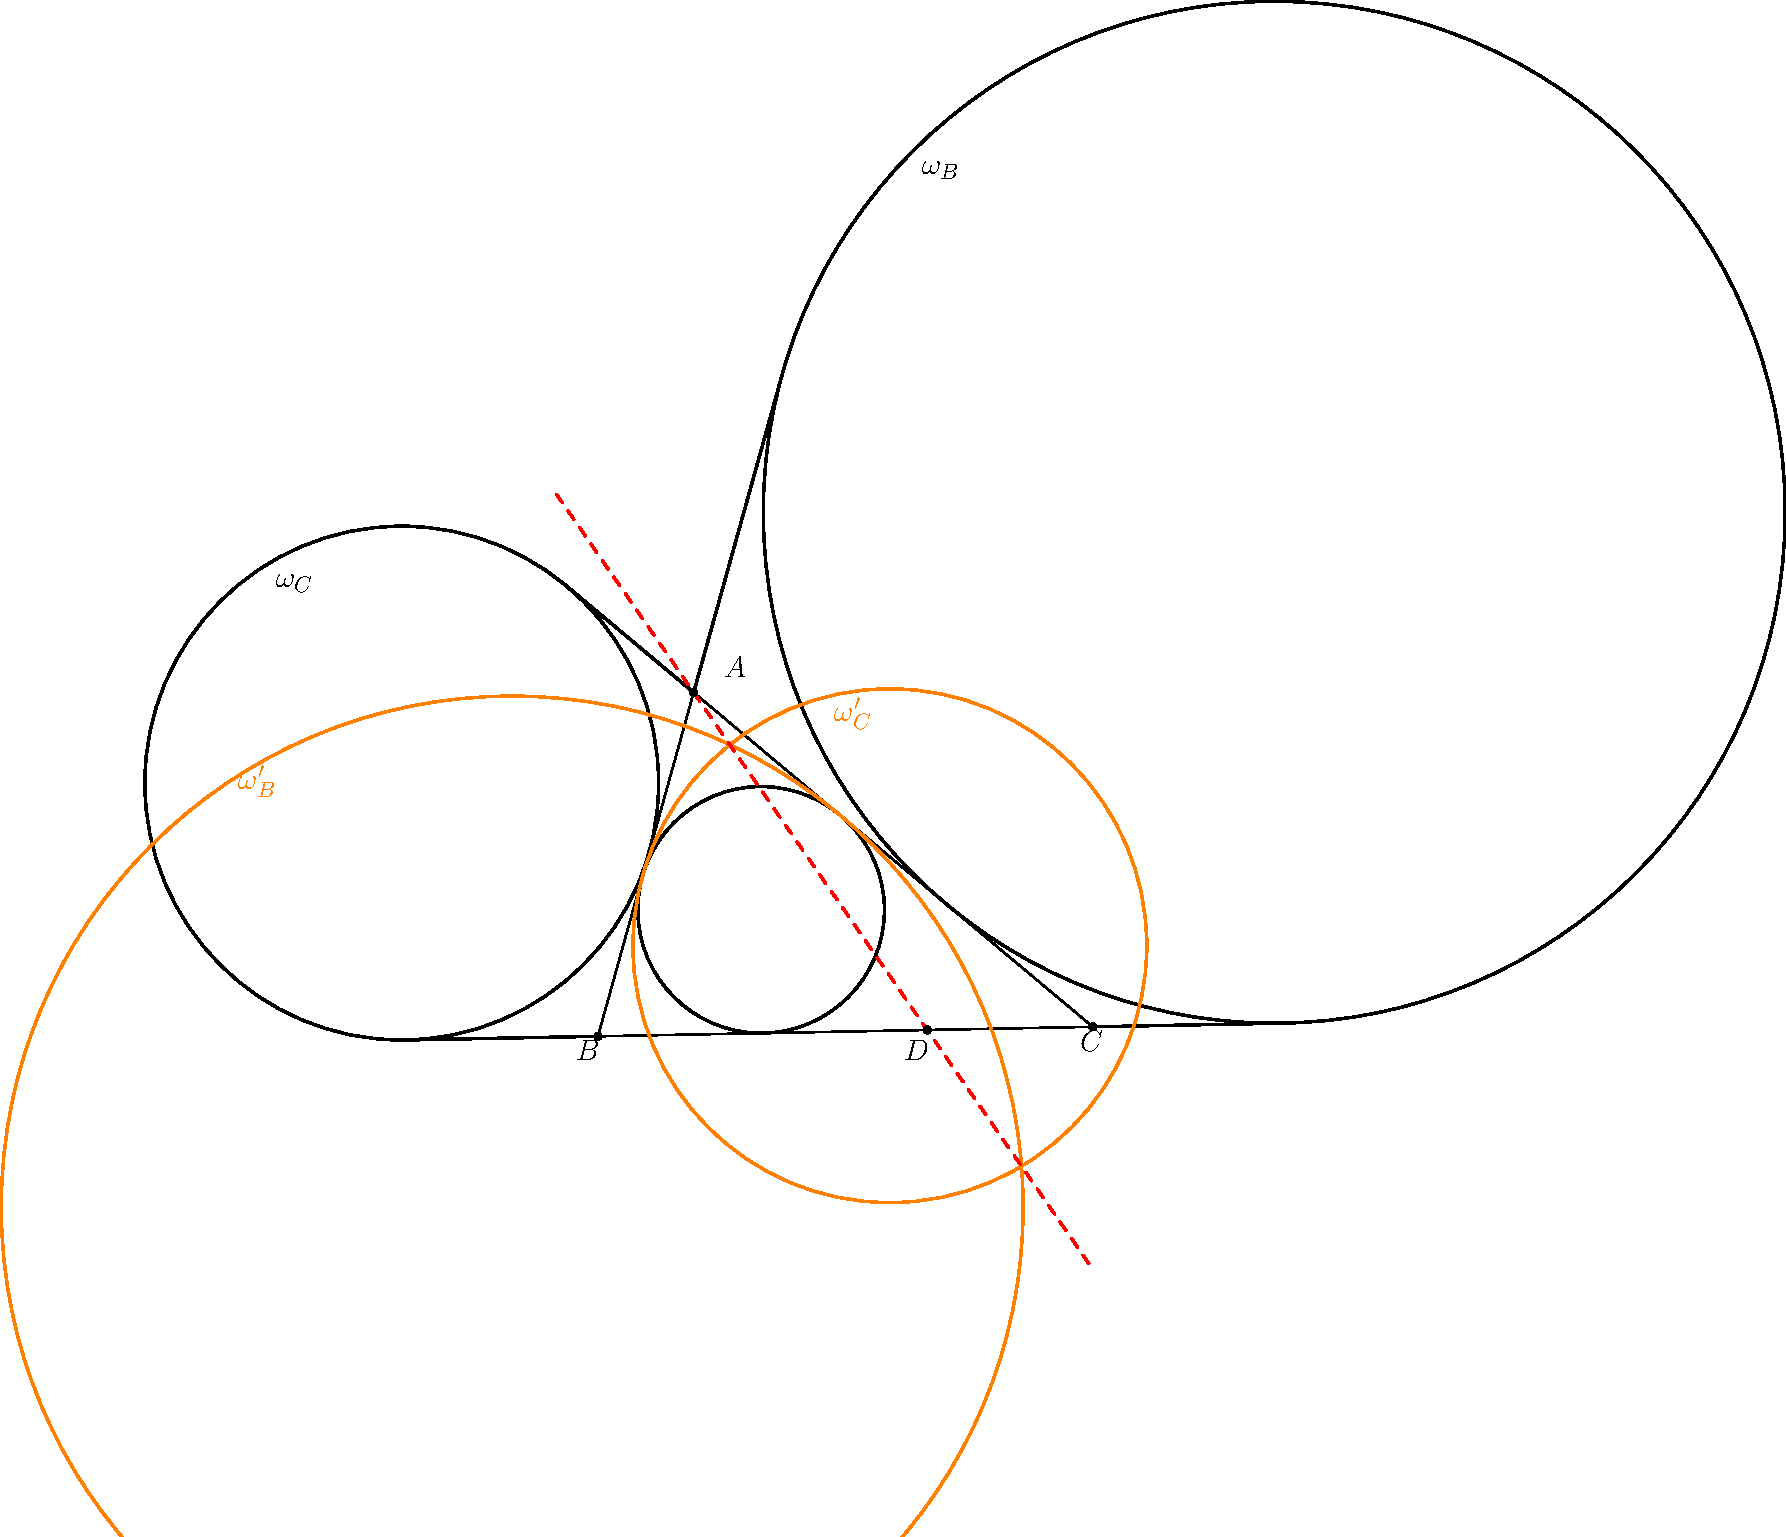
\includegraphics[width=.85\linewidth]{Figures/alrussian.pdf}
     % \caption{Caption}
     % \label{fig:enter-label}
 \end{figure}

 کافی است بگوییم که:
\[Pow_{\omega}^D-Pow_{\omega_B}^D=Pow_{\omega}^D-Pow_{\omega_C}^D\]
داریم:
\begin{align*}
Pow_{\omega}^D-Pow_{\omega_B}^D&=2 dist(D,\overline{AC}) (r_B-r) \\
&= 2 (p-b) Sin(\angle{ACB}) (r_B-r)
\end{align*}
به نحو مشابه داریم:
\[Pow_{\omega}^D-Pow_{\omega_C}^D=2 (p-c) Sin(\angle{ABC}) (r_C-r)\]
و در نهایت

\begin{align*}
2 (p-c) Sin(\angle{ABC}) (r_C-r)&=2 (p-b)Sin(\angle{ACB}) (r_B-r)\\
\Longleftrightarrow \frac{b}{c}&= \frac{(p-b)(r_B-r)}{(p-c)(r_C-r)} \thickspace (*)
\end{align*}

از طرفی داریم:
\[
\frac{r_B-r}{r}=\frac{c}{p-c} \thickspace \frac{r_c-r}{r}=\frac{b}{p-c}
\]
حالا با تقسیم این دو عبارت بر هم درستی $(*)$ را نتیجه میگیریم.
}



\section{اختلاف قوت}
\Th{\AfterTheorem
فرض کنید که دوایر $\omega_1$  $\omega_2$ و نقاط همخط $A$ ،$B$ و $C$ در یک صفحه هستند. و $C=\alpha A+(1-\alpha)B$ آنوقت داریم:
\[\mathbf{P}(C,\omega_1,\omega_2)=\alpha \mathbf{P}(A,\omega_1,\omega_2)+(1-\alpha)\mathbf{P}(B,\omega_1,\omega_2)\]

}


\Proof{
فرض کنید که $d_P$ فاصله نقطه $P$ تا محور اصلی $\omega_1$ و $\omega_2$ باشد. 

 \begin{figure}[!ht]
     \centering
     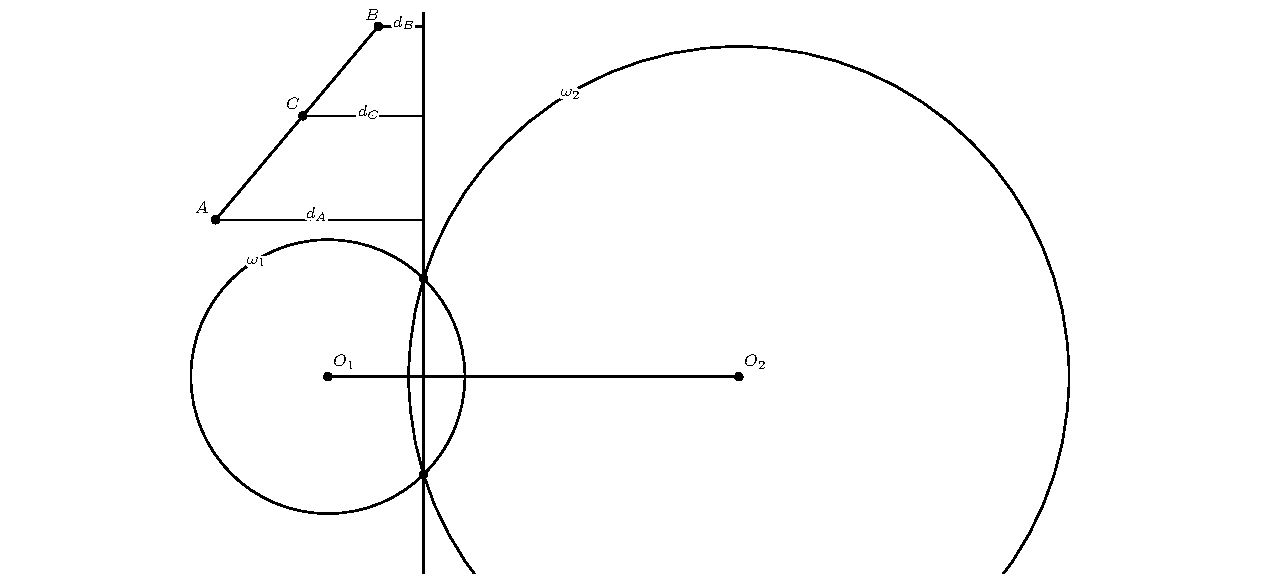
\includegraphics[width=.9\linewidth]{Figures/dif.pdf}
     % \caption{Caption}
     % \label{fig:enter-label}
 \end{figure}

حالا از قضیه \textbf{کیسی} داریم:
\begin{align*}
\mathbf{P}(C,\omega_1,\omega_2)=2d_cO_1O_2&=\frac{BC}{AB} \times \overbrace{2 d_A O_1O_2}^{\mathbf{P}(A,\omega_1,\omega_2)}+\frac{AC}{AB} \times \overbrace{2 d_B O_1O_2}^{\mathbf{P}(B,\omega_1,\omega_2)}\\
&= \alpha \mathbf{P}(A,\omega_1,\omega_2)+(1-\alpha) \mathbf{P}(B,\omega_1,\omega_2)
\end{align*}
که به این ترتیب حکم اثبات میشود.
}

\Ex{
چهاضلعی $APBQ$ در دایره $\omega$ محاط شده است به طوری که $\angle P=\angle Q=90^\circ$ و $AP=AQ<BP$. فرض کنید که $X$ نقطه ای متغیر بر روی پاره خط $\overline{PQ}$ باشد. خط $AX$، دایره $\omega$ را برای بار دیگر در نقطه $S$ قطع میکند. نقطه $T$ به روی کمان $AQB$ از $\omega$ قرار دارد به طوری که $\overline{XT}$ بر $\overline{AX}$ عمود است. اثبات کنید که اگر $M$ را وسط $\overline{ST}$ بنامیم، با حرکت $X$ روی پاره خط $\overline{PQ}$ مکان هندسی $M$ یک دایره است.

}

\Proof{
دایره به قطر $AO$ را $\omega'$ در نظر بگیرید. اثبات میکنیم که $M$ به روی دایره ای هم مرکز با $\omega'$ قرار دارد. برای این منظور کافی است اثبات کنیم قوت $M$ نسبت به $\omega'$ مستقل از $X$ است.
\begin{figure}[!ht]
     \centering
     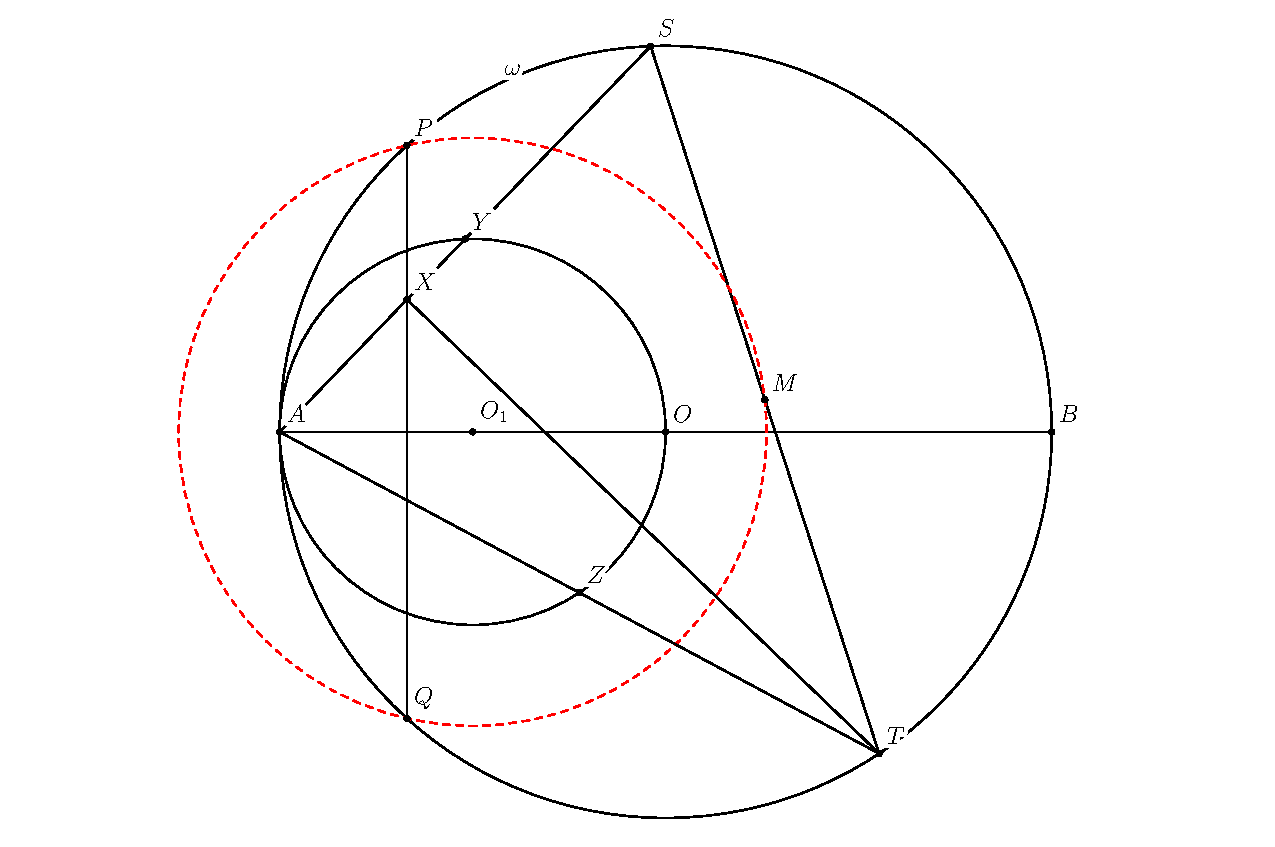
\includegraphics[width=\linewidth]{Figures/usa2015.pdf}
     % \caption{Caption}
     % \label{fig:enter-label}
 \end{figure}
بر اساس خطی بودن قوت نقطه میتوانیم بنویسیم:

\begin{align*}
    \mathbf{P}(M,\omega',\omega)&=(\frac12)\mathbf{P}(S,\omega',\omega)+(\frac12)\mathbf{P}(T,\omega',\omega)\\
    \implies Pow_M^{\omega'}&=\frac{AS^2+AT^2-ST^2}{4}\\
    &= \frac{2 AS \cdot AT \cos{(\angle A)}}{4}\\
    &=\frac{AP^2}{2}
\end{align*}
پس قوت $M$ نسبت به $\omega'$ برابر با ثابت $\frac{AP^2}{2}$ که نتیجه میدهد $M$ بر روی دایره ای به مرکز وسط $AO$ حرکت میکند.

}

\Le{
[نسبت قوت]
\AfterLemma
فرض کنید که دوایر $\omega_1$ و $\omega_2$ در صفحه موجود اند و برای نقطه $P$ مقدار $\frac{Pow_{\omega_1}^P}{Pow_{\omega_2}^P}$ ثابت است. آنوقت مکان هندسی نقاط $P$ با این خاصیت دایره ای است هم محور با $\omega_1$ و $\omega_2$.
}

\Proof{
فرض میکنیم که $X$ و $Y$ محل برخورد دو دایره $\omega_1$ و $\omega_2$  باشند. و $O'$،$O_1$ و $O_2$ به ترتیب مرکز دوایر $(PXY)$، $\omega_1$ و $\omega_2$ هستند. $l$ را هم محور اصلی $\omega_1$ و $\omega_2$ معرفی میکنیم. ادعا میکنیم که $O'$ ساکن است، چون اگر چنین باشد $P$ نیز بر روی دایره ای ثابت حرکت میکند.

\begin{figure}[!ht]
     \centering
     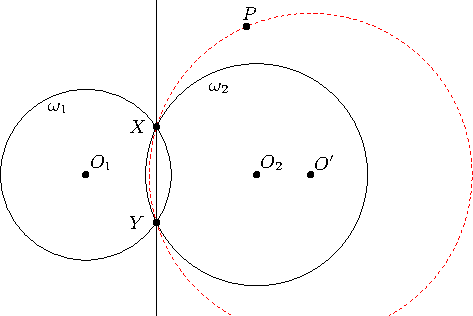
\includegraphics[width=0.7\linewidth]{Figures/powerratio.pdf}
     % \caption{Caption}
     % \label{fig:enter-label}
 \end{figure}


حال با دو بار استفاده از قضیه کیسی داریم:
\begin{align*}
    \begin{rcases}
    \mathbf{P}(P,(PXY),\omega_1)=2 dist (P,l)O'O_1 &=Pow_{\omega_1}^P \\ \mathbf{P}(P,(PXY),\omega_2)=2 dist (P,l)O'O_2 &=Pow_{\omega_2}^P
    \end{rcases} \implies \frac{Pow_{\omega_1}^P}{Pow_{\omega_2}^P}=\frac{O_1O'}{O_2O'}
\end{align*}

بنا بر این نسبت $\frac{O_1O'}{O_2O'}$ ثابت است که با توجه به جهت $P$ فقط میتوان یک نقطه برای $O'$ در نظر گرفت.
}

\Ex{
فرض کنید نقطه $P$ نقطه ای در صفحه مثلث $\triangle ABC$ است. و خط $l$ خطوط $BC$، $AC$ و $AB$ به ترتیب در نقاط $D$، $E$ و$F$ قطع میکند.
$A'$ را محل برخورد خط $AP$ با $l$ و نقاط $B'$ و $C'$ را به همین ترتیب تعریف میکنیم.
اثبات کنید که دوایر $(PDA')$ ، $(PEB')$ و $(PFC')$ در نقطه ی دیگری به غیر از $P$ برخورد دارند.
}


\Proof{
دایره $(PA'D)$ را $\omega_A$ مینامیم و $\omega_B$ و $\omega_C$ را به نحو مشابه تعریف میکنیم. 

\begin{figure}[!ht]
     \centering
     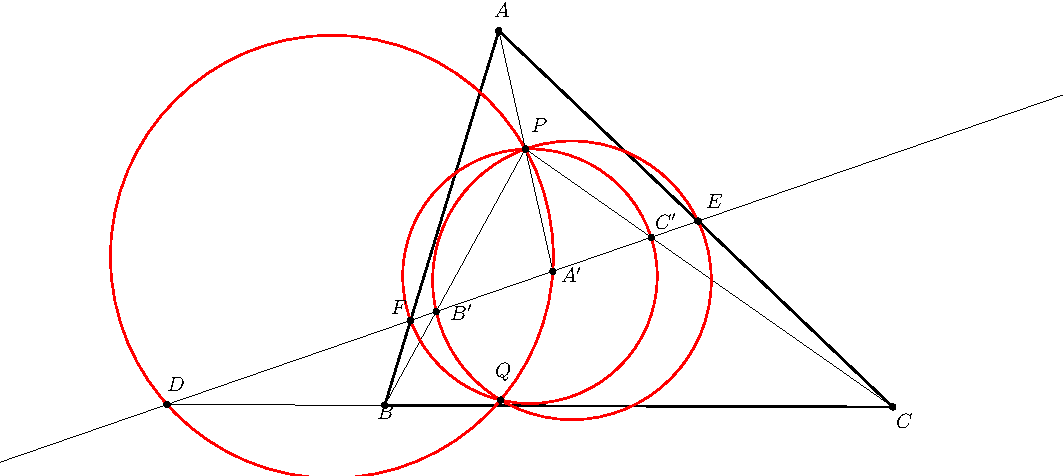
\includegraphics[width=0.85\linewidth]{Figures/powerratioexam.pdf}
     % \caption{Caption}
     % \label{fig:enter-label}
 \end{figure}

\newpage
دایره $(PA'D)$ را $\omega_A$ مینامیم و $\omega_B$ و $\omega_C$ را به نحو مشابه تعریف میکنیم. حالا کافی است اثبات کنیم که $\frac{Pow_{\omega_B}^A'}{Pow_{\omega_C}^A'}=
\frac{Pow_{\omega_B}^D}{Pow_{\omega_C}^D}$ زیرا برا اساس لم نسبت قوت میتوانیم نتیجه بگیریم که $D$ و $A'$ برو روی دایره ای قرار دارند که از قضا با دوایر $\omega_B$ و $\omega_C$ هم محور است و ما را به نتیجه مطلوب میرساند.
بنا بر این داریم:
\begin{align*}
    \frac{Pow_{\omega_B}^D}{Pow_{\omega_C}^D} &= \frac{Pow_{\omega_B}^{A{'}}}{Pow_{\omega_C}^{A{'}}}\\
\iff  \frac{DB' . DE}{DF . DC'} &= \frac{A'B' . A'E}{A'C' . A'F} \\ 
\iff \frac{\frac{DB'}{DC'}}{\frac{A'B'}{A'C'}}&=\frac{\frac{DE}{DF}}{\frac{A'E}{A'F}} \thickspace (*)
\end{align*}
حال با استفاده از ناهمساز ادامه میدهیم:
\[LHS=(DA',B'C')\stackrel{P}{=} (D \overline{AP}\cap \overline{BC},BC)\stackrel{A}{=} (DA',FE)=RHS\] 
}

\Le{
[لم هم محوری]\AfterLemma

اگر $َABCD$ چهارضلعی محاطی باشد و  خط $l$ خطوط $AD$ و $BC$ را در $P$ و $Q$ قطع کنند و داشته باشیم $\angle{BQP}=\angle{APQ}$  و اگر خطوط $AC$ و $BD$ را در $S$ و $R$ قطع کند. آنوقت دایره ای که از $P$ و $S$ میگذرد و بر اقطار چهارضلعی مماس است ، دایره ای که از $P$ و $Q$ میگذرد و  بر اضلاع چهارضلعی مماس است و دایره محیطی $(ABCD)$ هم محور اند.
}
\Proof{

اولا واضح است که دایره ای وجود دارد که در $R$ و $S$ بر قطر ها مماس باشد چون داریم:
\[
\angle CSQ=180^{\circ} - \angle SQC-\angle BCA=180^{\circ}-\angle ADB-\angle DPR=\angle DRP
\]


\begin{center}
\definecolor{ffxfqq}{rgb}{1.,0.4980392156862745,0.}
\definecolor{qqwuqq}{rgb}{0.,0.39215686274509803,0.}
\begin{tikzpicture}[line cap=round,line join=round,>=triangle 45,x=5.0cm,y=5.0cm]
\clip(-1.191089412812065,-0.9126328878674588) rectangle (1.0472556143556455,1.1182979282885712);
\draw [shift={(-0.870089509413483,0.09908328195144034)},line width=0.pt,,color=qqwuqq,fill=qqwuqq,fill opacity=0.30000001192092896] (0,0) -- (5.491201803936025:0.08642258792153322) arc (5.491201803936025:79.74305460440165:0.08642258792153322) -- cycle;
\draw [shift={(0.4200153517807076,0.22310631205285036)},line width=0.pt,,color=qqwuqq,fill=qqwuqq,fill opacity=0.30000001192092896] (0,0) -- (111.23934900347041:0.08642258792153322) arc (111.23934900347041:185.49120180393606:0.08642258792153322) -- cycle;
\draw [shift={(-0.14635299479559077,0.1686590181864451)},line width=0.pt,,color=ffxfqq,fill=ffxfqq,fill opacity=0.30000001192092896] (0,0) -- (-41.16200053320602:0.08642258792153322) arc (-41.16200053320602:5.491201803936026:0.08642258792153322) -- cycle;
\draw [shift={(-0.5574287853955602,0.1291406296545637)},line width=0.pt,,color=ffxfqq,fill=ffxfqq,fill opacity=0.30000001192092896] (0,0) -- (-174.508798196064:0.08642258792153322) arc (-174.508798196064:-127.85559585892197:0.08642258792153322) -- cycle;
\draw [line width=0.4pt] (-0.04033054103004885,0.011523011722871068) circle (5.cm);
\draw [line width=0.4pt] (-0.760362029331924,0.7054644039555197)-- (-0.9578838334606404,-0.3860898094358302);
\draw [line width=0.4pt] (0.11852063546094307,0.9988255508300222)-- (0.7435679726205908,-0.6093659640983444);
\draw [line width=0.4pt] (-0.760362029331924,0.7054644039555197)-- (0.11852063546094307,0.9988255508300222);
\draw [line width=0.4pt] (0.7435679726205908,-0.6093659640983444)-- (-0.9578838334606404,-0.3860898094358302);
\draw [line width=0.4pt] (0.11852063546094307,0.9988255508300222)-- (-0.9578838334606404,-0.3860898094358302);
\draw [line width=0.4pt] (-0.760362029331924,0.7054644039555197)-- (0.7435679726205908,-0.6093659640983444);
\draw [line width=0.4pt,domain=-1.191089412812065:1.0472556143556455] plot(\x,{(--0.18188996845907746--0.09569290084947672*\x)/0.9954109044645897});
\draw [line width=0.4pt] (-0.33324027341721635,-0.04510649265913878) circle (1.4197055023636993cm);
\draw [line width=0.4pt] (-0.20755018757925736,-0.02080628519000752) circle (3.366496180325767cm);
\begin{scriptsize}
\draw [fill=black] (-0.760362029331924,0.7054644039555197) circle (1.5pt);
\draw[color=black] (-0.7935455083730122,0.7625249413449262) node {$A$};
\draw [fill=black] (0.11852063546094307,0.9988255508300222) circle (1.5pt);
\draw[color=black] (0.14846069997169994,1.0563617402781393) node {$B$};
\draw [fill=black] (0.7435679726205908,-0.6093659640983444) circle (1.5pt);
\draw[color=black] (0.7822263447296102,-0.6576862534989358) node {$C$};
\draw [fill=black] (-0.9578838334606404,-0.3860898094358302) circle (1.5pt);
\draw[color=black] (-1.012482731107563,-0.4329875249029495) node {$D$};
\draw [fill=black] (-0.870089509413483,0.09908328195144034) circle (1.5pt);
\draw[color=black] (-0.8914911080174165,0.17197059054778283) node {$P$};
\draw [fill=black] (0.4200153517807076,0.22310631205285036) circle (1.5pt);
\draw[color=black] (0.4394167459741951,0.284319954845776) node {$Q$};
\draw [fill=black] (-0.5574287853955602,0.1291406296545637) circle (1.5pt);
\draw[color=black] (-0.5746082856384613,0.20077811985496055) node {$R$};
\draw [fill=black] (-0.14635299479559077,0.1686590181864451) circle (1.5pt);
\draw[color=black] (-0.1367338401693597,0.2382279079542916) node {$S$};
\end{scriptsize}
\end{tikzpicture}
\end{center}

حالا توجه کنید که $\triangle BQR \sim \triangle APS$ و $\triangle QSC \sim \triangle PRD$ پس داریم:

\[\frac{AP}{AS}=\frac{BQ}{BR}=\frac{\sin(\angle BRQ)}{\sin(\angle BQR)}=\frac{\sin(\angle CSQ)}{\sin(\angle CQS)}=\frac{CQ}{CS}=\frac{DP}{DR}\]


پس در نتیجه نسبت قوت نقاط $A$، $B$، $C$ و $D$ نسبت به دو دایره کوچکتر ثابت است بنابراین روی دایره ای هم محور با دو دایره کوچکتر قرار دارن. که این حکم را نتیجه میدهد.

}

\section{قضیه کیسی (برای دوایر)}

\Th{
[قضیه کیسی]\AfterTheorem
مثلث $\triangle ABC$ مفروض است. و دایره ی $\omega$ در صفحه مفروض است. $AD$، $BE$ و $CF$ مماس های وارد بر دایره ی $\omega$ هستند. رابطه ی:
\[AD\cdot BC\pm BE\cdot AC \pm CF \cdot AB=0\]
برقرار است اگر و تنها اگر $(ABC)$ و $\omega$ بر هم مماس باشند.
}
\Proof{
ابتدا طرف اگر را اثبات میکنم. فرض کنید که دو دایره $(ABC)$ و $\omega$ در نقطه $T$ مماس باشند.

\begin{center}{
\begin{tikzpicture}[line cap=round,line join=round,>=triangle 45,x=4.0cm,y=4.0cm]
\clip(-1.1811104846600597,-1.1008238345724661) rectangle (1.1347959344142975,1.1153912485814719);
\draw [line width=1.2pt] (0.,0.) circle (4.cm);
\draw [line width=1.2pt] (-0.01242000448386445,-0.6336276649202868) circle (1.4650024875319048cm);
\draw [line width=1.2pt] (-0.4120598809876899,0.9111567672362484)-- (-0.9993928721630809,-0.034840882159149225);
\draw [line width=1.2pt] (-0.9993928721630809,-0.034840882159149225)-- (0.9999909723064365,-0.004249153518957376);
\draw [line width=1.2pt] (-0.4120598809876899,0.9111567672362484)-- (0.9999909723064365,-0.004249153518957376);
\draw [line width=1.2pt] (-0.4120598809876899,0.9111567672362484)-- (-0.3785855404026436,-0.6415218612049083);
\draw [line width=1.2pt] (-0.9993928721630809,-0.034840882159149225)-- (-0.2919222428025695,-0.8703089206303675);
\draw [line width=1.2pt] (0.9999909723064365,-0.004249153518957376)-- (-0.10087001536506998,-0.2782178822682311);
\begin{scriptsize}
\draw [fill=black] (-0.4120598809876899,0.9111567672362484) circle (2.0pt);
\draw[color=black] (-0.4679340046139828,0.994611360831733) node {$A$};
\draw [fill=black] (-0.9993928721630809,-0.034840882159149225) circle (2.0pt);
\draw[color=black] (-1.0852534308904258,-0.06748479493581172) node {$B$};
\draw [fill=black] (0.9999909723064365,-0.004249153518957376) circle (2.0pt);
\draw[color=black] (1.0619445735493758,-0.0061362805232459475) node {$C$};
\draw [fill=black] (-0.01959765944191752,-0.9998079474301045) circle (2.0pt);
\draw[color=black] (-0.003985864368954324,-0.9186954324101616) node {$T$};
\draw [fill=black] (-0.3785855404026436,-0.6415218612049083) circle (2.0pt);
\draw[color=black] (-0.32606556503492456,-0.5889471674426207) node {$D$};
\draw [fill=black] (-0.2919222428025695,-0.8703089206303675) circle (2.0pt);
\draw[color=black] (-0.23787707556686127,-0.8113355321881716) node {$E$};
\draw [fill=black] (-0.10087001536506998,-0.2782178822682311) circle (2.0pt);
\draw[color=black] (-0.11901432889251512,-0.18634754161015785) node {$F$};
\end{scriptsize}
\end{tikzpicture}
} \end{center}

میتوانیم $T$ را نقطه ای هم محور با دو دایره دیگر در نظر بگیریم بنابر این طبق لم نسبت قوت، ثابت $c\neq 0$ وجود دارد که:

\[ \frac{AD}{AT}=\frac{BE}{BT}=\frac {CF}{CT}=c \]
پس طبق فرض داریم:
\[
AD\cdot BC\pm BE\cdot AC \pm CF \cdot AB=c(AT\cdot BC\pm BT\cdot AC \pm CT\cdot AB)=0
\]
که چون $ABTC$ محاطی است طبق قضیه بطلمیوس این رابطه برقرار است. حالا برعکس قضیه را اثبات میکنیم. فرض کنید که دو دایره مماس نیستند و این رابطه برقرار است. $T$ را نقطه ای در نظر بگیرید که با دو دایره $(ABC)$ و $\omega$ هم محور باشد. دوباره طبق لم نسبت قوت، ثابت $c\neq 0$ وجود دارد که:
\[
AD\cdot BC\pm BE\cdot AC \pm CF \cdot AB=c(AT\cdot BC\pm BT\cdot AC \pm CT\cdot AB)=0
\]
اما اگر $AT\cdot BC\pm BT\cdot AC \pm CT\cdot AB=0$ طبق قضیه بطلمویس $T$ باید روی دایره ی $(ABC)$ باشد که این نتیجه میدهد که دو دایره ی $(ABC)$ و $\omega$ بر هم مماس اند.

}

\Ex{
ثابت کنید که در هر مثلثی دایره ی نه نقطه بر دایره محاطی آن مثلث مماس است.

}

\Proof{
با استفاده از قضیه کیسی بر مثلث $\triangle MNP$ حکم را اثبات میکنیم:
\begin{center}
\definecolor{qqqqff}{rgb}{0.,0.,1.}
\begin{tikzpicture}[line cap=round,line join=round,>=triangle 45,x=4.0cm,y=4.0cm]
\clip(-1.31613673265523,-1.3706287340998176) rectangle (1.3526697121828377,1.1832953141061473);
\draw [line width=1.2pt] (0.,0.) circle (4.cm);
\draw [line width=1.2pt] (-0.38346843174658946,0.9235539842661128)-- (-0.9986731646922362,0.051496700123343536);
\draw [line width=1.2pt] (-0.9986731646922362,0.051496700123343536)-- (0.9986042655654797,0.052815914215593764);
\draw [line width=1.2pt] (-0.38346843174658946,0.9235539842661128)-- (0.9986042655654797,0.052815914215593764);
\draw [line width=1.2pt] (-0.28341670878659386,0.42253765985929287) circle (1.4822737903624152cm);
\draw [line width=1.2pt] (-0.191768665436673,0.5139332993025251) circle (2.cm);
\draw [line width=2.pt,color=qqqqff] (-0.6910707982194129,0.48752534219472815)-- (-0.5862189388356198,0.6361536326399977);
\draw [line width=2.pt,color=qqqqff] (-0.2831719460890527,0.05196929310231779)-- (-3.444956337828042E-5,0.052156307169468646);
\draw [line width=2.pt,color=qqqqff] (0.30756791690944507,0.48818494924085326)-- (-0.08588453123139549,0.7360691784981876);
\draw [line width=1.2pt] (0.30756791690944507,0.48818494924085326)-- (-0.6910707982194129,0.48752534219472815);
\draw [line width=1.2pt] (-3.444956337828042E-5,0.052156307169468646)-- (-0.6910707982194129,0.48752534219472815);
\draw [line width=1.2pt] (-3.444956337828042E-5,0.052156307169468646)-- (0.30756791690944507,0.48818494924085326);
\begin{scriptsize}
\draw [fill=black] (-0.38346843174658946,0.9235539842661128) circle (1.5pt);
\draw[color=black] (-0.45010020419784386,1.0087624422996844) node {$A$};
\draw [fill=black] (-0.9986731646922362,0.051496700123343536) circle (1.5pt);
\draw[color=black] (-1.0952090468242641,0.005750748627099525) node {$B$};
\draw [fill=black] (0.9986042655654797,0.052815914215593764) circle (1.5pt);
\draw[color=black] (1.0698822743192014,0.041099178360054056) node {$C$};
\draw [fill=black] (-3.444956337828042E-5,0.052156307169468646) circle (1.5pt);
\draw[color=black] (5.922748973265484E-4,-0.03843478853909364) node {$M$};
\draw [fill=black] (0.30756791690944507,0.48818494924085326) circle (1.5pt);
\draw[color=black] (0.33640235736039464,0.5536514094878948) node {$N$};
\draw [fill=black] (-0.6910707982194129,0.48752534219472815) circle (1.5pt);
\draw[color=black] (-0.7638175180778153,0.5271400871881788) node {$P$};
\draw [fill=black] (-0.2831719460890527,0.05196929310231779) circle (1.5pt);
\draw[color=black] (-0.29545082411616774,0.138307360125679) node {$D$};
\draw [fill=black] (-0.08588453123139549,0.7360691784981876) circle (1.5pt);
\draw[color=black] (-0.13638289031787226,0.681789467269855) node {$E$};
\draw [fill=black] (-0.5862189388356198,0.6361536326399977) circle (1.5pt);
\draw[color=black] (-0.5561454933967074,0.5713256243543721) node {$F$};
\end{scriptsize}
\end{tikzpicture}
\end{center}

\begin{align*}MD\cdot NP\pm NE\cdot MP\pm PF \cdot MN &= \frac{b-c}{2}\cdot \frac{a}{2} - \frac{a-c}{2} \cdot \frac{b}{2} + \frac{a-b}{2} \cdot \frac{c}{2} \\
&=\frac{ba-ca-ab+bc+ac-bc}{4}\\
&=0 \end{align*}

بنابر این طبق قضیه کیسی دایره ی محاطی و دایره نه نقطه بر هم مماس اند.

}

\section {سوالات پایان فصل}
\EnumAlph{
\Prob{ \link{https://artofproblemsolving.com/community/u485879h1737106p22557407}{KöMaL A. 733}
دایره $\omega$ درون دایره $\Omega$ قرار دارد و نقطه $X$ روی $\Omega$ حرکت می‌کند. خطوط مماس از $X$ به $\omega$ برخورده دوم با دایره $\Omega$ را در نقاط $A\neq X$ و $B\neq X$ قرار می‌دهند. ثابت کنید خطوط $AB$ یا همگی به یک دایره ثابت مماس هستند یا همگی از یک نقطه عبور می‌کنند.
}

\Prob{\link{https://artofproblemsolving.com/community/c6h1610595p10055973}{RMM 2017}
چهارضلعی محدب $ABCD$ و نقاط دلخواه $P$ و $Q$ در داخل آن را در نظر بگیرید بطوری که $\angle APB = \angle CPD = \angle AQB = \angle CQD$ باشد. ثابت کنید که خط های $PQ$ بدست آمده از این روش، همگی از یک نقطه ثابت می گذرند یا همگی موازی اند.
}

\Prob{
\link{https://artofproblemsolving.com/community/c5h532234p3041822}{USAMO 2013}
در مثلث $ABC$ نقاط $P$ ، $Q$ و $R$ به ترتیب روی اضلاع $BC$ ، $CA$ و $AB$ قرار دارند. $\omega_A$ و$\omega_B$ ،$\omega_C$ به ترتیب دایره های محیطی مثلث های $AQR$ ، $BRP$ و $CPQ$ هستند.  
با این فرض که پاره خط $AP$ ، $\omega_A$ و$\omega_B$ ،$\omega_C$ را دوباره به ترتیب در $X$ ، $Y$ و $Z$ قطع کند، ثابت کنید $YX/XZ = BP/PC$.
}
\Prob{
در مثلث $ABC$  نقطه ی $D$ روی ضلع $BC$ انتخاب شده است.دایره محیطی مثلث های $ABD$ و $ACD$ اضلاع $AC$  و $AB$ را به ترتیب در نقاط $E$ و $F$ قطع می‌کند.ثابت کنید با تغییر $D$ روی ضلع $BC$, دایره محیطی $AEF$ از نقطه ثابتی میگذرد.و این نقطه روی میانه ی گذرنده از $A$ می‌باشد.}

\Prob{دایره های $(O_1)$ و $(O_2)$ به ترتیب در نقاط $M$ و $N$ از داخل به دایره ی مفروض $(O)$ مماس هستند. 
مماس های داخلی مشترک این دو دایره، دایره ی $(O)$ را در 4 نقطه قطع می کنند، 
نقاط $B$ و $C$ را دو نقطه از این نقاط در نظر بگیرید بطوری که $B$ و $C$ هر دو در یک سمت خط $O_1O_2$ باشند.  
ثابت کنید که $BC$ با یک مماس خارجی مشترک $(O_1)$ و $(O_2)$ موازی است.}

\Prob{فرض کنید $\Omega$ دایره محیطی $ABC$ و نقطه ی $D$ نقطه ی اشتراک $BC$ با دایره محاطی مثلث $ABC$ باشد.فرض کنید $\omega$ دایره ای درون $\Omega$  مماس باشد که و در نقطه ی $D$ بر $BC$ باشد.ثابت کنید $\angle ATI = 90$}

\Prob{
دوایر $\omega_A$،$\omega_B$ و $\omega_C$ با مراکز همخط $A$، $B$ و $C$ موجودند.$g$ خطی است که از این سه نقطه میگذرد. $X$ محل برخورد محور اصلی $\oemga_B$ و $\omega_C$ با $g$است. به همین ترتیب $Y$ محل برخورد محور اصلی $\omega_A$ و $\omega_C$ با خط $g$ و $Z$ محل برخورد محور اصلی $\omega_A$ و $\omega_B$ با $g$ است. رابطه ی زیر را اثبات کنید:
\[
\overline{YZ}=\frac{1}2 ( \frac{x^2}{\overline{AB}\cdot \overline{AC}}+\frac{y^2}{\overline{BC} \cdot \overline{BA}}+\frac{z^2}{\overline{CA}\cdot \overline{CB}} ) \cdot \overline{BC}
\]
}

\Prob{
دایره ی $\omega$ و نقطه ی $T$ خارج آن مفروض اند. $A$ و $B$ برخورد مماس های وارده از $T$ بر $\omega$ اند. نقطه ی $P$ بر روی کمان کوچکتر $AB$ قرار دارد. از طرفی داریم $E=AP\cap RB$ و $F=AT\cap BP$. $Q$ نقطه ی دوم برخورد دو دایره ی $(AFP)$ و $(PBE)$ است.ثابت کنید:
\[\angle POT=|\angle TAP-\angle TBP|\] 

}
\Prob{\link{https://artofproblemsolving.com/community/c6h1264730p6580553}{USA TSTST 2016}
فرض کنید $\triangle ABC$ یک مثلث با مرکز دایره محاطی $I$ باشد و دایره محاطی آن به ترتیب بر $\overline{BC}$, $\overline{CA}$, $\overline{AB}$ در $D$، $E$ و $F$ مماس باش. فرض کنید $K$ پای ارتفاع از $D$ بر $\overline{EF}$ باشد. فرض کنید که دایره $\triangle AIB$ با دایره محاطی در دو نقطه مجزا $C_1$ و $C_2$ ملاقات کند، در حالی که دایره  $\triangle AIC$ با دایره محاطی در دو نقطه مجزا $B_1$ و $B_2$ ملاقات کند. ثابت کنید که محور اصلی دایره‌های $\triangle BB_1B_2$ و $\triangle CC_1C_2$ از وسط $\overline{DK}$ میگذرد.
}
\Prob {

مثلث $\triangle ABC$ مفروض است. $I$ مرکز دایره محاطی آن و نقطه ی $D$ بر روی خط $BC$ به طور دلخواه انتخاب شده است. $\omega_1$ دایره ای است که بر دو پاره خط $AD$ و $BD$ و $(ABC)$ از داخل محاط است. دایره ی $\omega_2$ هم به نحو مشابه بر $\overline{AD}$، $\overline{CD}$ و $(ABC)$ از داخل مماس است. دایره های $\omega_1$ و $\omega_2$ به ترتیب در نقاط $P$ و $Q$ بر $\overline{BC}$ مماس اند. ثابت کنید که وسط کمان کوچکتر $BC$ روی $(ABC)$، وسط $PQ$ و وسط $ID$ همخط اند.

}


\Prob{

مثلث $\triangle ABC$ مفروض است. نقاط $E$ و $F$ بر روی اضلاع $AC$ و  $AB$ قرار دارند به طوری که بر دایره محاطی $\triangle ABC$ مماس اند، $BC\neq EF$ و $BC\mid \mid EF$. ثابت کنید دایره ای وجود دارد که از دو نقطه $B$ و $C$ بگذرد و بر دو دایره ی محاطی مثلث های $\triangle ABC$ و $\triangle AEF$ مماس باشد.

}
\newpage
\Prob{

مثلث $\triangle ABC$ مفروض است. دایره ی $(I_A)$ دایره ی میکستیلینیر متناظر به $A$ در این مثلث است و $M$ وسط کمان کوچک تر $BC$ است. اگر $T$ محل برخورد مماس از $M$ بر $(I_A)$ باشد ثابت کنید:
\[
\frac{MT}{MA}=|\frac{b-c}{b+c}|
\]

}

\Prob{
\link{https://artofproblemsolving.com/community/q1h1876745p21109392}{IMO 2019}
مثلث $\triangle ABC$ به همراه دایره محاطی اش $(I)$ مفروض است. $(I)$ بر $BC$، $AC$ و $AB$ در $D$، $E$ و $F$ مماس است. ارتفاع وارده از $D$ بر خط $EF$، $(I)$ را برای بار دوم در $R$ قطع میکند. خط $AR$، $(I)$ را برای بار دوم در $P$ قطع میکند. دوایر $(PCE)$ و $(PBF)$ یکدیگر را برای بار دوم در $Q$ قطع میکنند.
ثابت کنید که خطوط $DI$ و $PQ$ یکیدیگر را روی نیمساز خارجی زاویه ی $\angle ABC$ قطع میکنند.

}


\Prob{
\link{https://artofproblemsolving.com/community/q1h2803071p24709975}{AOPS}
مثلث $\triangle ABC$ به همراه دایره محاطی اش $(I)$ مفروض است. $(I)$ بر $BC$، $AC$ و $AB$ در $D$، $E$ و $F$ مماس است. $AD$، $BE$ و $CF$ دایره ی $(I)$ را برای بار دوم در $X$، $Y$ و $Z$ قطع میکنند. دوایر $(\omega_A)$، $(\omega_B)$ و $\omega_C$ از $A$، $B$ و $C$ میگذرند و بر $(I)$ به ترتیب در $X$، $Y$ و $Z$ مماس اند. اگر $Ge$ نقطه ی ژرگون مثلث $\triangle ABC$ باشد، ثابت کنید که مرکز قوت دوایر $(\omega_A)$، $(\omega_B)$ و $\omega_C$ بر روی خط $IGe$قرار دارد.

}

}


\end{document}
